\chapter{Part F: Credit Curve}
Developer: Aloke Mukherjee

\noindent Validator: Yann Renoux


%DEVELOPER WRITES THIS PART --->

\section{Requirements}

%<description of the problem being solved, relevant equations, algorithms, etc>
A credit curve is similar to a yield curve in that it can be used to
calculate discount factors and thus present or future values of a
risky security.  The key difference is that there is a spread at
each maturity between the credit curve and the yield curve
corresponding to the additional return required for taking on the
added risk.

Credit curves are associated with the issuer's creditworthiness.
There is always a probability that the issuer will default and thus
be unable to meet their debt obligations.  A survival probability
quantifies the probability at any given time that the issuer will
"survive" to meet these obligations.  Survival probability declines
with time and declines faster for less credit-worthy issuers.

We calculate implied probabilities from credit default swap spreads.
In a credit swap the buyer of protection pays the spread
periodically and the seller pays in the event of a default.  These
two legs must have equal present values.  The assumption underlying
this model is that the spread on a risky asset vs. a non-risky asset
is entirely compensation for the possibility of default.  The
CreditCurve class models the modified yield curve as well as the
issuer's survival probability, hazard rate and recovery rate.

\section{Design }

All of the discounting functionality can be reused from the
YieldCurve object.  The CreditCurve object must also maintain a
collection of spread points.

The more interesting part of the implementation was bootstrapping
the default probabilities.  We decided to implement the calculation
recursively.  We define the following terms:

$q_{n}$ - default intensity.  This is the probability of default in
period n conditional on no earlier default.

$Q_{n}$ - default probability.  This is the probability of default in
period n as seen from time 0.

$S_{n}$ - survival probability.  This is the chance of survival to
time n.

$C_{n}$ - cumulative default probability.  This is the chance of
default before time n.  It is the complement of $S_{n}$.  This value
is called $Q_{n}$ in Professor Laud's notes.

$F_{n}$ - fees associated with one leg of a credit default swap.
Both legs are assumed equal to this value so the quantity can be
computed either from the perspective of the buyer or seller of
protection.

$B(0,t_{n})$ - discount factor.  The value of one dollar received at
time $t_{n}$.

$s_{n}$ - spread.  The credit spread over the riskfree rate at
time n.

$R$ - recovery rate.  The proportion of face value recovered in
the event of default.  It is usually assumed to be 40\%.

The following relationships hold for these quantities:

$$q_{0} = 0, q_{1} = Q_{1}$$

$$Q_{2}=(1-q_{1})(q_{2}) \Rightarrow Q_{n} = (\prod_{i=1}^{n-1}(1-q_{i}))q_{n}$$

$$S_{n} = 1 - \sum_{i=1}^{n}Q_{i} = \prod_{i=1}^{n}(1 - q_{i})$$

$$C_{n} = 1 - S_{n} = \sum_{i=1}^{n}Q_{n}$$

Generalizing from the risk-neutral argument of equality between swap
legs at each default time we can write down the following recursive
formula for $q_{n}$ in terms of fees $F_{n}$, survival probabilities $S_{n}$, spreads $s_{n}$,
recovery rate $R$ and appropriate discount factors:

$$q_{n}=\frac{F_{n-1}(\frac{s_{n}}{s_{n-1}} - 1) + B(0,t_{n}) s_{n} S_{n-1}}{B(0,t_{n}) S_{n-1} (1 - R + s_{n})}, q_{0} = 0 (probability\ of\ default\ at\ time\ 0\ is\ 0\%)$$

$$S_{n}=S_{n-1} (1 - q_{n}), S_{0} = 1 (probability\ of\ survival\ at\ time\ 0\ is\ 100\%)$$

$$F_{n}=F_{n-1} \times \frac{s_{n}}{s_{n-1}} + B(0,t_{n}) s_{n} S_{n-1} (1 - q{n})$$

$$F_{0} = 0 (no\ fees\ at\ time\ 0)$$

By implementing recursive methods for default probability, survival
probability and fees we can calculate default intensities at
discrete time intervals.  Notice that all the above is considered in
the discrete time setting for simplicity of implementation and
because of the discrete nature of the spread data.

\section{Choices}
%<any important design choices you made, e.g. data structures, class hierarchy, algorithm, etc. and a justification for the decision>

There are three choices with respect to reuse of the YieldCurve
class.  CreditCurve can inherit from YieldCurve, YieldCurve and
CreditCurve could both inherit from some common class or CreditCurve
could contain a YieldCurve.

The first two have the benefit of allowing polymorphism - e.g. a
function designed to take a YieldCurve object and use it for
discounting can also take a CreditCurve object.  This would not be
possible in the third case unless there were some method of
CreditCurve which returned a YieldCurve.  This is cumbersome.  Of
the two polymorphic approaches the first has the benefit of
simplicity and intuitiveness: namely there is no object more basic
than a YieldCurve in finance and secondly the CreditCurve is a type
of YieldCurve rather than a type of some other more basic object.
Our implementation takes the first approach.

In calculating default probabilities we decided to throw out the .5
year spread since keeping it requires having a special case. Instead
we standardize the calculation on 1 year intervals - i.e. we assume
that defaults happen at the 1/2 year mark.  Another justification
for this is that looking at the sample data we received for AIG from
Bloomberg, it appears that the .5 year spread is interpolated (equal
to 1 year spread).


\begin{figure}
\begin{center}
        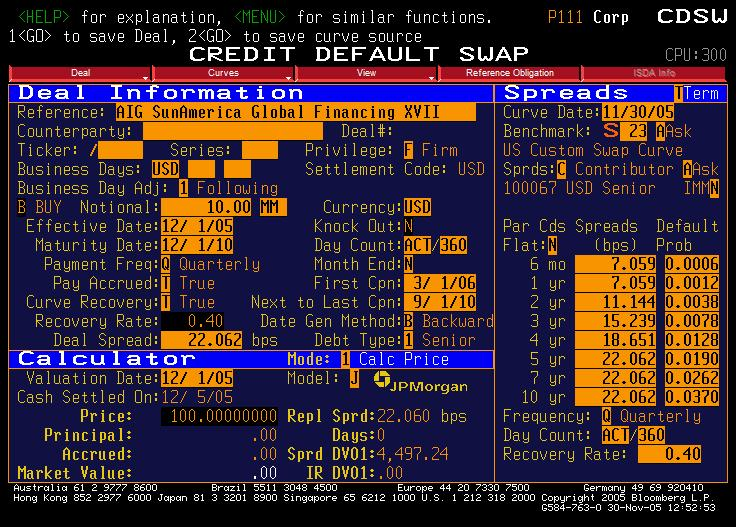
\includegraphics[width=10cm]{CDSW_AIG.jpg}
        \caption{Bloomberg CDS data for AIG}
\end{center}
\end{figure}

We also decided to internally interpolate spreads at 1 year
granularity rather than working with discontinuities in the spread
data.  Hull suggests one approach for calculating default
probabilities on an interval where there is no spread data: assume a
constant unconditional default probability in each period.  Since
the calculations implemented here work with conditional default
probabilities it is easier to assume a spread and leave the
calculation as it is.  From the rough relationship $$h =\frac{s}{(1-R)}$$ 
we know that spreads are proportional to
conditional default probabilities.  So interpolating spreads is like
assuming a constant default probability in the interval.  The
approach of using a constant default intensity is suggested in
section 21.3 of OFOD (6th edition). For another supporting argument
for this approach see
http://www.fincad.com/newsletter.asp?i=1140\&a=1800 which suggests
interpolating CDS spreads as an improvement vs. constant "default
density" (a.k.a. unconditional default probabilities).

The risky discount factor was calculated by multiplying the
underlying riskfree discount factor by the discrete time survival
probability up to that time rather than using a continuous
hazard-rate function.  In the class notes we have $RF = DF \times
(1 - Q(T))$.  $Q(T)$ is cumulative default probability (in
Professor Laud's notes, here we denote it $C_{n}$) so it is the
complement of $S(T)$, the cumulative survival probability.

In discrete time we have the identity: $\frac{(S_{n} -
S_{n+1})}{S_{n}} = q_{n}$.  $q_{n}$ is a discrete time version of
hazard rate.  In the limit this leads to the expression $S(t) =
exp(-\int_0^th(t)dt)$.

The risky discount factor is a "discounted" discount factor - the
discounting applied is the survival probability. In continuous time
we can use the expression above but since we have calculated
everything to this point in discrete time and we have an explicit
expression for the survival probability we use this as the discount
factor rather than the continuous time expression above.

\section{Unit tests}
%<short descriptions of each subtest>

The recursive algorithm was first implemented in Matlab.  The
M-files can be found in the data directory: $$defprob.m, survprob.m,
fees.m$$ Using Matlab some of the results in section 21 of OFOD
were successfully reproduced.  When implemented in C++ the results
were verified against the Matlab output as well as the example in
OFOD.  Another source of verification was the reuse of the credit
curve class in implementing the risky bond.

Additionally the given data for AIG was encoded in a file and used
to instantiate a CreditCurve.  The data was gathered using
CreditCurve's appropriate methods and plotted here and on the
following pages. The cumulative default probability curve comes
quite close to the Bloomberg curve.

\begin{figure}
\begin{center}
        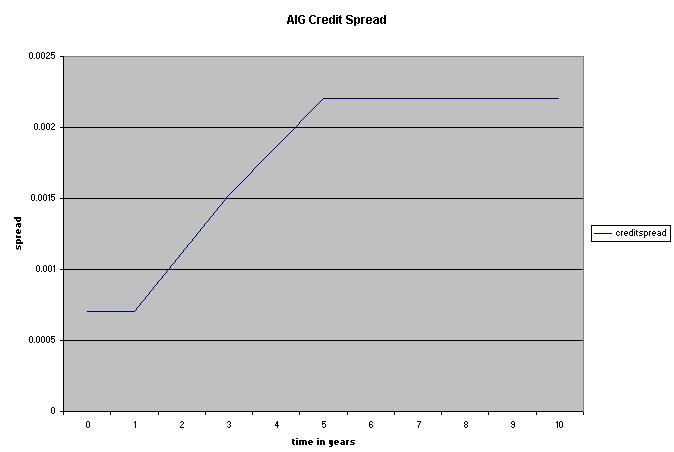
\includegraphics[width=10cm]{creditcurve-spread.jpg}
        \caption{Credit spreads}
\end{center}
\end{figure}


\begin{figure}
\begin{center}
        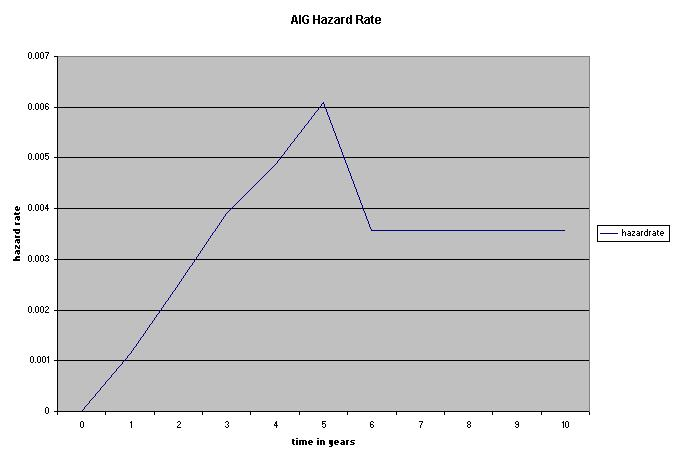
\includegraphics[width=10cm]{creditcurve-hazardrate.jpg}
        \caption{$q_{n}$ - hazard rate or default intensity}
\end{center}
\end{figure}


\begin{figure}
\begin{center}
        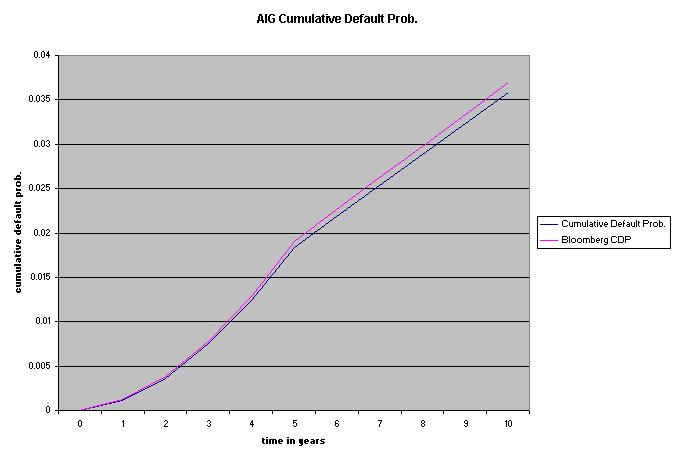
\includegraphics[width=10cm]{creditcurve-cumdefaultprob.jpg}
        \caption{Comparison between calculated and values from Bloomberg}
\end{center}
\end{figure}

\begin{figure}
\begin{center}
        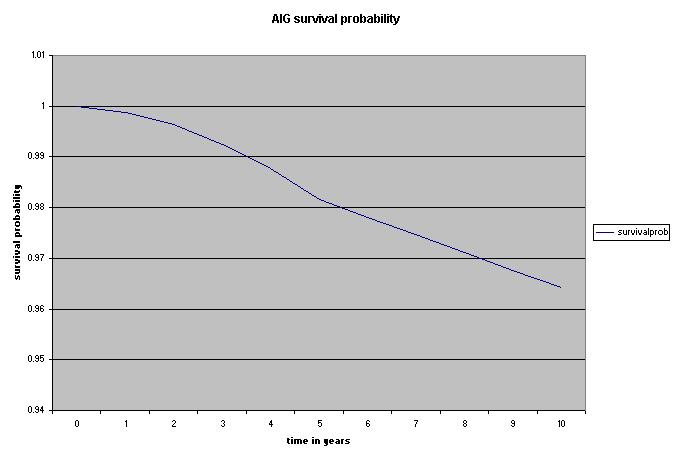
\includegraphics[width=10cm]{creditcurve-survivalprob.jpg}
        \caption{Survival probability}
\end{center}
\end{figure}

\begin{figure}
\begin{center}
        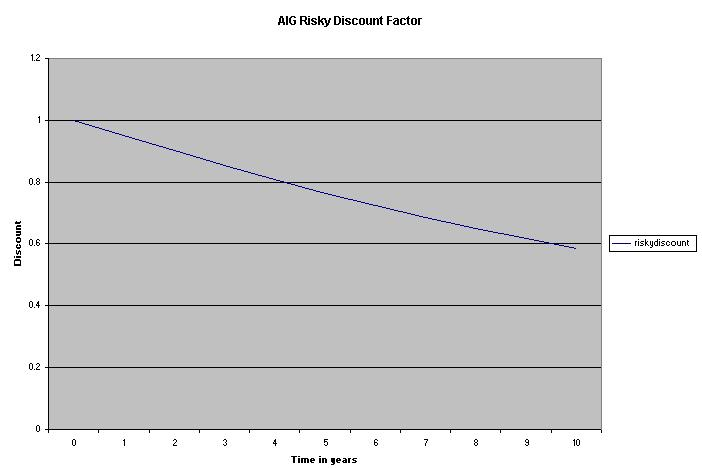
\includegraphics[width=10cm]{creditcurve-riskydiscount.jpg}
        \caption{The risky discount factor}
\end{center}
\end{figure}

\section{Performance}

%<how can the performance of this component be sped up by 100%?>
Recursion can be time-consuming resulting in many nested calls.  One
approach to improving performance is to cache intermediate results.
Caching was implemented and makes the performance O(n) for the first
call (assuming you are calculating default probabilities from
earlier to later periods).  Once all values are cached, results are
immediate.  Overhead for the first call could be further reduced if
the values were cached at construction.

The best candidate for performance improvement in the CreditCurve
class is probably the method used to construct the curve.  The
spreads are all converted to relative spreads and then used to
construct a new yield curve. Then the spotrates of the underlying
curve and the "spread curve" are summed to instantiate a combined
curve.  This procedure is a bit overly time and memory consuming and
could be optimized.

%VALIDATOR WRITES THIS PART --->

\section{Validation}


\subsection{Approach}

We applied the algorithm present in Pr. Laud lecture notes. Define
\begin{itemize}
    \item A spread $sprd_T$ is paid annually constantly to protect for the default during $T$ years.
    \item $q_i =q(i-1,i)$ is the conditional probability of default in period i. $q_0=1$
    \item $Q(i)$ is the cumulative probability such as $Q(0)=0$ and $Q(i+1)=Q(i)+q_{i+1}[1-Q(i)]$
\end{itemize}

To compute we note that the Present Value of the fees on the whole
life should equal the loss occurred in case of default, all been on
the point of view of the seller. If we call $B(0,j)$ the risk free
discount factor up to year $j$ and $R$ the recovery rate:

\begin{eqnarray*}
    \mathbb{E}(PVFees,T)&=&sprd_T\times\sum_{i=1}^T\left(B(0,i)\prod_{j=1}^i(1-q_j)\right)\\
    \mathbb{E}(Loss,T)&=&(1-R)\times\sum_{i=1}^T\left(q_iB(0,i)\prod_{j=1}^{i-1}(1-q_{j})\right)\\
\end{eqnarray*}

The first conditional probability is easy to compute, and we used Excel's "Goal Seek" to find recursively the conditional probabilities that would equal the fees and the loss. We repeated this for 5 years -- credit spreads were provided by the developper and we used the default yield curve, and were led to the $Q(i)$ which are used to get the risky discount factor. The results are as follows:

\begin{center}
\begin{tabular}{|l|l|l|l|l|l|l|}
\cline{3-7}
\multicolumn{1}{l}{} & \multicolumn{1}{c|}{} & \multicolumn{3}{c|}{Values of Q(i) computed with several tools} & \multicolumn{2}{c|}{Relative Differences between Q(i)'s} \\
\hline
Yr & \multicolumn{1}{c|}{creditspread} & \multicolumn{1}{c|}{Terreneuve} & \multicolumn{1}{c|}{Excel} & \multicolumn{1}{c|}{BBG (Interpolation)} & \multicolumn{1}{c|}{Excel/Bloomberg} & \multicolumn{1}{c|}{ Excel/TN} \\
\hline
$1$ & \multicolumn{1}{c|}{$0.00071$} & \multicolumn{1}{c|}{$0.00115$} & \multicolumn{1}{c|}{$0.00118$} & \multicolumn{1}{c|}{$0.0012$} & \multicolumn{1}{c|}{$2.1\%$} & \multicolumn{1}{c|}{$2.4\%$} \\
\hline
$2$ & \multicolumn{1}{c|}{$0.00111$} & \multicolumn{1}{c|}{$0.00365$} & \multicolumn{1}{c|}{$0.00374$} & \multicolumn{1}{c|}{$0.0038$} & \multicolumn{1}{c|}{$1.6\%$} & \multicolumn{1}{c|}{$2.4\%$} \\
\hline
$3$ & \multicolumn{1}{c|}{$0.00152$} & \multicolumn{1}{c|}{$0.00754$} & \multicolumn{1}{c|}{$0.00772$} & \multicolumn{1}{c|}{$0.0078$} & \multicolumn{1}{c|}{$1.0\%$} & \multicolumn{1}{c|}{$2.3\%$} \\
\hline
$4$ & \multicolumn{1}{c|}{$0.00187$} & \multicolumn{1}{c|}{$0.01237$} & \multicolumn{1}{c|}{$0.01266$} & \multicolumn{1}{c|}{$0.0128$} & \multicolumn{1}{c|}{$1.1\%$} & \multicolumn{1}{c|}{$2.3\%$} \\
\hline
$5$ & \multicolumn{1}{c|}{$0.00221$} & \multicolumn{1}{c|}{$0.01839$} & \multicolumn{1}{c|}{$0.01881$} & \multicolumn{1}{c|}{$0.0190$} & \multicolumn{1}{c|}{$1.0\%$} & \multicolumn{1}{c|}{$2.2\%$} \\
\hline
\end{tabular}
\end{center}

The differences are not very important, as in relative value $2\%$, but still significative. Neither TN nor Excel matches Bloomberg results, which explains by the fact that we did not have the yield curve of the same day of quotation of the CDS. We still have to mention that Excel seems closer to Bloomberg, but that TN results are far from being off, so the class can be validated as it is and consider giving a fair result for all the objects that use it. Once this works, the formulas exposed before follow form one another.

\begin{figure}
\begin{center}
        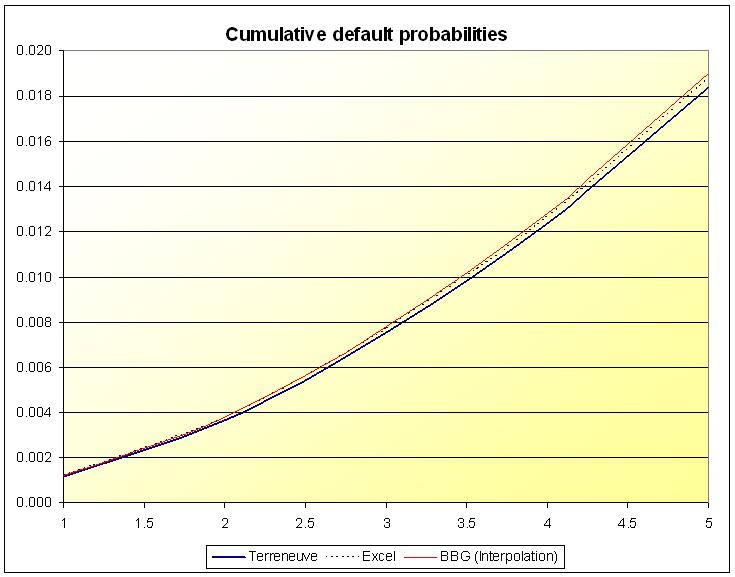
\includegraphics[width=14cm,height=10cm]{CumDefProbasYann.jpg}
        \caption{Cumulative default probabilities -- BBG vs TN vs Validation}
\end{center}
\end{figure}

Also, the object seems to be created really properly, and all tests of methods produce an expected behaviour for reasonnable inputs.
